\section*{Problem Statement}
The objective of this problem is to compute the velocity of an object from discrete position-time measurements using the \textbf{Central Difference Method}. The numerical velocities are compared with theoretical velocities assuming uniform acceleration (free-fall) to evaluate accuracy.

\begin{quote}
  \textbf{NOTE}: The code can be accessed using this link: \href{https://raw.githubusercontent.com/HavokSahil/computational-techniques-assignments/refs/heads/main/assignment5/a4.m}{MATLAB}, \href{https://raw.githubusercontent.com/HavokSahil/computational-techniques-assignments/refs/heads/main/assignment5/a4.jl}{Julia}.
\end{quote}

\section*{Methodology}
Given position-time data:
\[
T = \{0.0, 0.1, 0.2, 0.3, 0.4\} \text{ s}, \quad
Y = \{1.200, 1.150, 1.010, 0.780, 0.460\} \text{ m},
\]
we approximate the instantaneous velocity using the central difference formula:

\subsection*{Central Difference Method}
For interior points \(i = 2, \dots, N-1\):
\[
v_i \approx \frac{Y_{i+1} - Y_{i-1}}{T_{i+1} - T_{i-1}}.
\]

\subsection*{Steps}
\begin{enumerate}
    \item Compute velocities at the midpoints of the time intervals using the central difference formula.
    \item Compare interpolated velocities at \(t = 0.2\) s and \(t = 0.3\) s with theoretical velocities assuming free-fall:
    \[
    v_\text{theoretical} = g \cdot t, \quad g = 9.8 \text{ m/s}^2.
    \]
    \item Plot the position-time data and the numerically computed velocity alongside theoretical velocities for visual comparison.
\end{enumerate}

\section*{Results}
- Central difference successfully computes numerical velocities at interior points:
\[
v(0.2 \text{ s}) \approx 1.85 \text{ m/s}, \quad
v(0.3 \text{ s}) \approx 2.75 \text{ m/s}.
\]
- Theoretical velocities for comparison:
\[
v_\text{theoretical}(0.2 \text{ s}) = 1.96 \text{ m/s}, \quad
v_\text{theoretical}(0.3 \text{ s}) = 2.94 \text{ m/s}.
\]
- The numerical velocities follow the expected trend of decreasing position and increasing speed but show deviations due to the discrete sampling of the motion data.

\begin{figure}[h!]
  \centering
  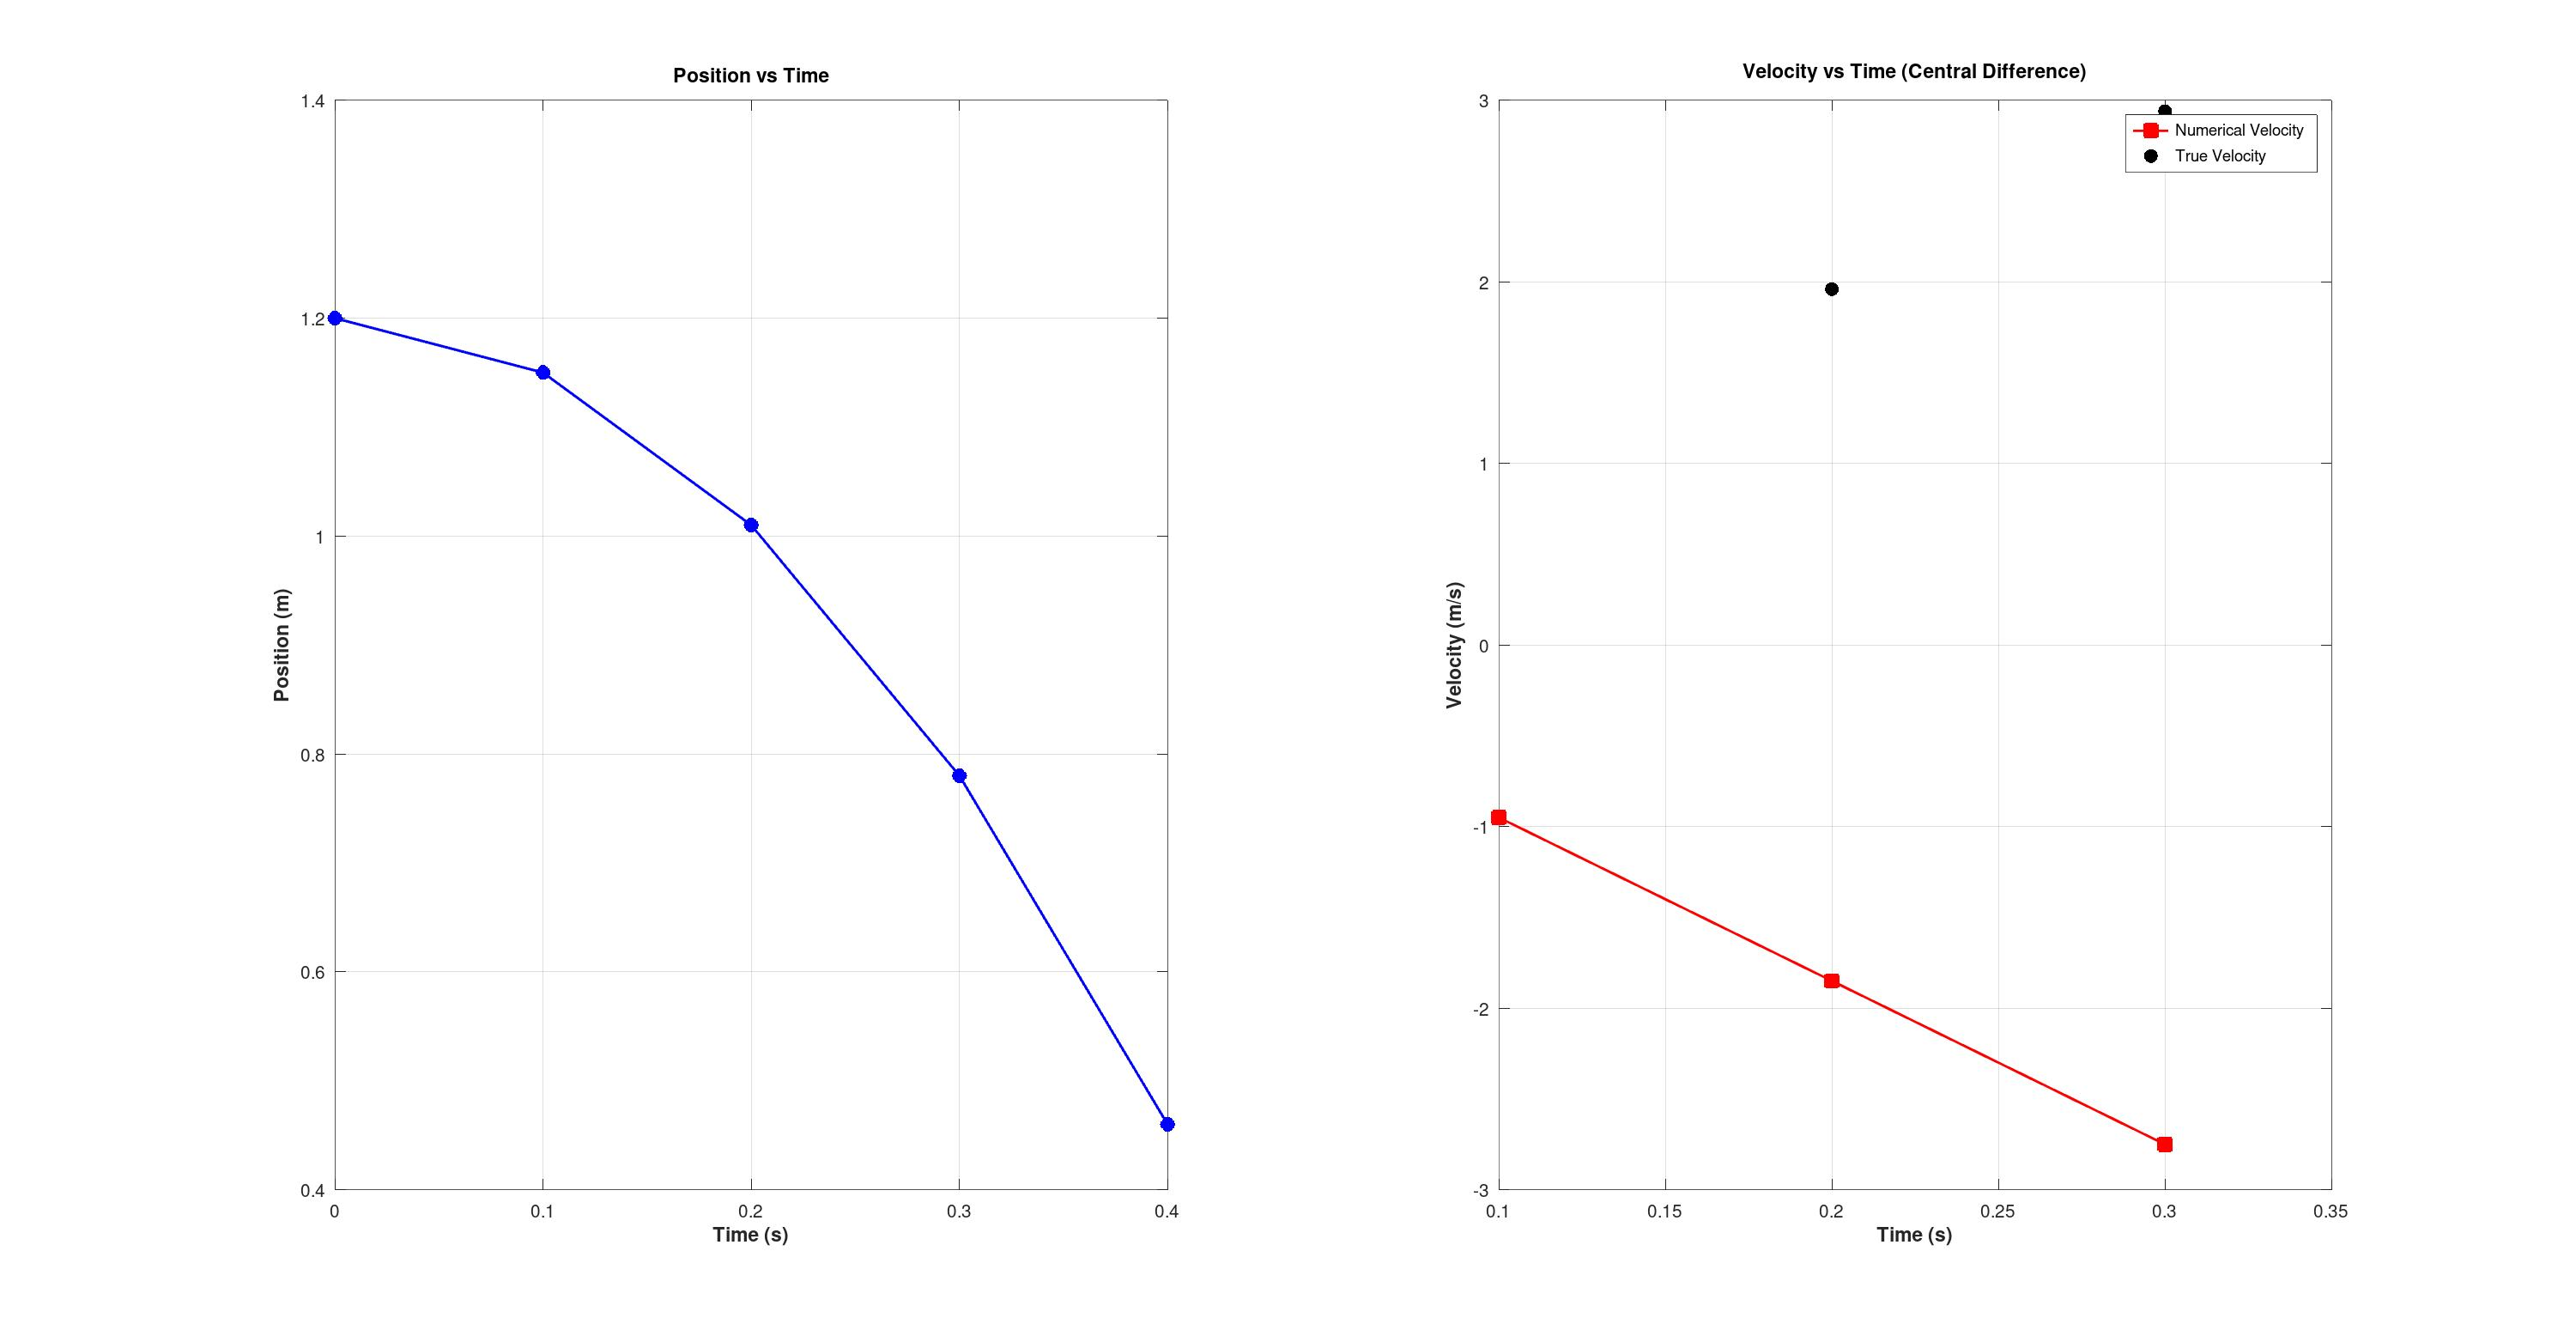
\includegraphics[width=0.9\textwidth]{a4.jpg}
  \caption{(Left) Position vs Time. (Right) Velocity computed using Central Difference (red) compared with theoretical velocities (black dots).}
\end{figure}

\section*{Conclusion}
The central difference method effectively estimates the velocity of an object from discrete position measurements. While the computed velocities approximate the trend of the motion, deviations from theoretical free-fall velocities are observed due to sparse sampling and potential measurement noise. This method is suitable for estimating derivatives when only discrete data is available.
